\usetikzlibrary{quotes,angles}
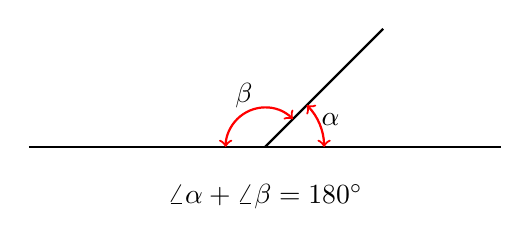
\begin{tikzpicture}[scale=1.5]
  %
  \coordinate (a) at (-2,0);
  \coordinate (o) at (0,0) node[below=1em] {$\angle \alpha + \angle \beta = 180^\circ$};
  \coordinate (c) at (1,1);
  \coordinate (d) at (2,0);
  %
  \draw[thick] (a) -- (o);
  \draw[thick] (o) -- (c);
  \draw[thick] (o) -- (d);
  %
  \draw pic["$\alpha$", thick, draw=red, <->, angle eccentricity=1.2, angle radius=0.75cm] {angle=d--o--c};
   \draw pic["$\beta$", thick, draw=red, <->, angle eccentricity=1.4, angle radius=0.5cm] {angle=c--o--a};
   
\end{tikzpicture}